\documentclass{beamer}
\usetheme{Madrid}

\usepackage{graphicx}

% ── Fill in your details ──────────────────────────────────────────
\newcommand{\thesistitle}{Privacy awareness in point clouds using AI-based object detection}
\newcommand{\theauthor}{George Fakidis}
\newcommand{\thesupervisor}{Prof. George Xylomenos}
\newcommand{\reviewerone}{Prof. George C. Polyzos}
\newcommand{\reviewertwo}{Prof. Vasilios A. Siris}
\newcommand{\thedate}{\today}
% ─────────────────────────────────────────────────────────────────
\title{\thesistitle}
\author{\theauthor}
\date{\thedate}
\setbeamerfont{author in head/foot}{size=\tiny}

\begin{document}
% \addbibresource{MSc-Thesis.bib}


\begin{frame}[plain]
	\centering
	
\includegraphics[width=0.25\textwidth]{figs/aueb_logo.jpg} % replace with your logo file
	\vspace{0.5cm}

	{\Large\bfseries \thesistitle \par}
	\vspace{0.5cm}

	{\large \theauthor \par}
	\vspace{0.8cm}

	\begin{columns}[t]
		\column{0.33\textwidth}
		\centering
		{\small\textbf{Supervisor} \\ \thesupervisor}

		\column{0.33\textwidth}
		\centering
		{\small\textbf{Reviewer} \\ \reviewerone}

		\column{0.33\textwidth}
		\centering
		{\small\textbf{Reviewer} \\ \reviewertwo}
	\end{columns}

	\vspace{0.8cm}
	{\small \thedate}
\end{frame}

% ── Add your slides below ─────────────────────────────────────────

\begin{frame}{Outline}
	\tableofcontents
\end{frame}

\section{Related Work}
\begin{frame}{Related Work}
	\cite{Zhao_Zhang_Demiris_2024} 3PFS: End-to-end pipeline for pedestrian privacy in 2D videos.
	\begin{figure}[htb]
		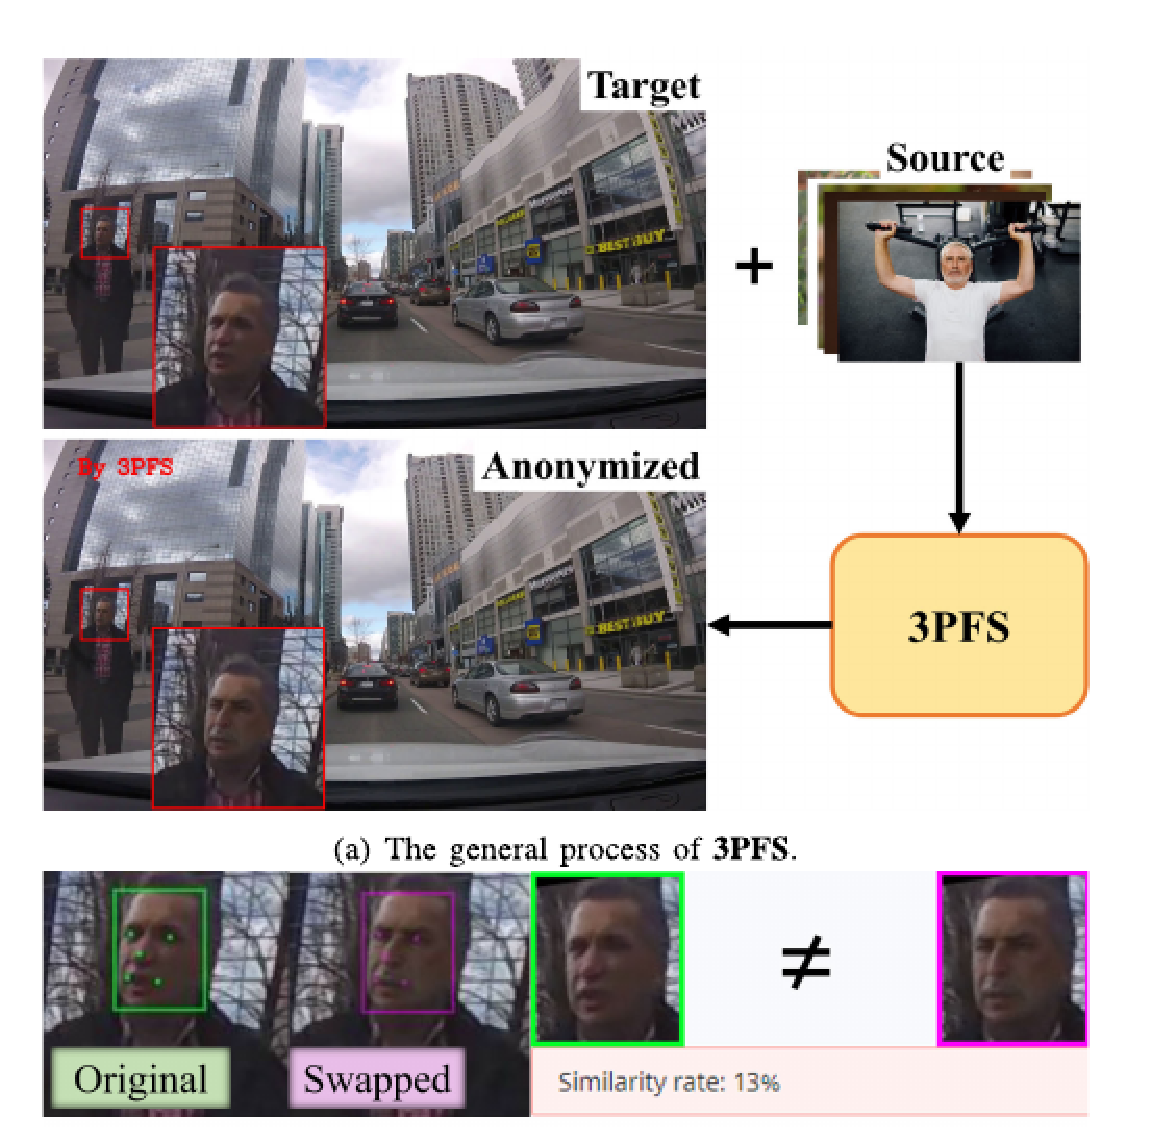
\includegraphics[width=\textwidth, height=0.7\textheight, keepaspectratio]{figs/3PFS-Related-Work.pdf}
	\end{figure}
\end{frame}

\section{3D Object Detection Models}
\begin{frame}{3D Object Detection Models}
	I can mention some models here, the most influential ones.
\end{frame}

\begin{frame}{Related Work}
	Enhanced privacy preservation work at: \cite{Kunchala_Bouroche_Schoen-Phelan_2023}
	\begin{figure}[htb]
		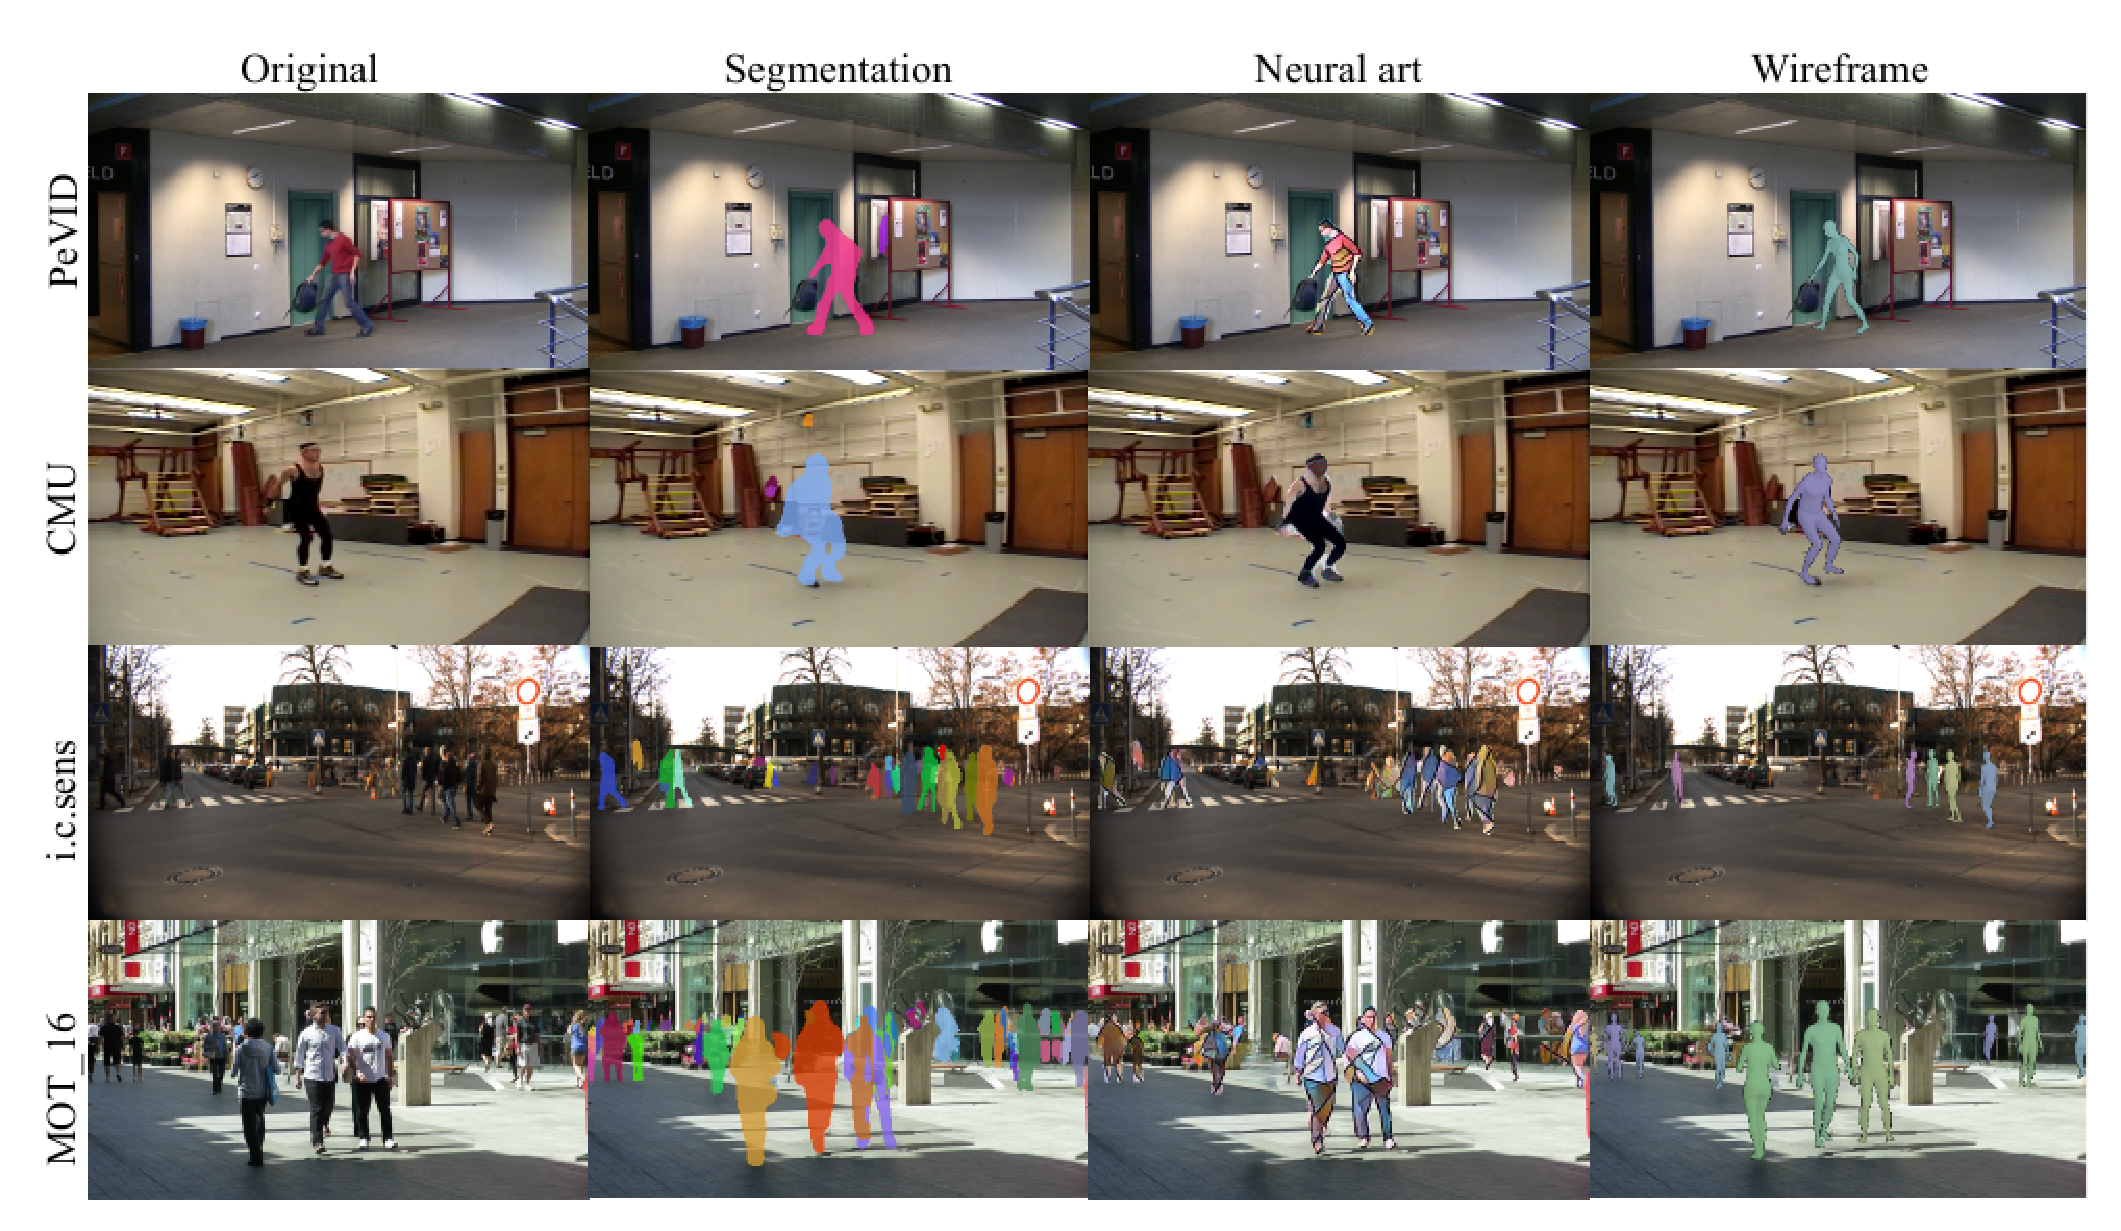
\includegraphics[width=\textwidth, height=0.7\textheight, keepaspectratio]{figs/anonymized-pedestrian-video-data.pdf}
	\end{figure}
\end{frame}

\section{Datasets}
\begin{frame}{Datasets for Point Cloud Object Detection}
	Most 3D detection datasets target autonomous driving captured by LiDAR. Note: pedestrians are a category but not faces.

	\begin{itemize}
		\item \textbf{KITTI} \cite{geiger_are_2012}: one of the earliest LiDAR benchmarks, classes: car, pedestrian, cyclist
		\item \textbf{ONCE} \cite{mao_one_2021}: 1 million LiDAR scenes, 15 annotated classes
		\item \textbf{Argoverse 2} \cite{wilson_argoverse_2023}: 26-category taxonomy including rare classes such as strollers, wheelchairs, and animals
		\item \textbf{JRDB} \cite{Martín-Martín_Patel_Rezatofighi_Shenoi_Gwak_Frankel_Sadeghian_Savarese_2023}: $\sim$1 hour of sensor data from a mobile robot, annotated with 3D bounding boxes for pedestrians
		\item \textbf{SUN RGB-D} \cite{Song_Lichtenberg_Xiao_2015}: 10,335 RGB-D images with 2D and 3D annotations across multiple sensors, suitable for general scene understanding
	\end{itemize}
\end{frame}

\begin{frame}{Datasets-Visual Overview}
	\begin{columns}[T]
		\column{0.4\textwidth}
		\begin{figure}
			\centering
			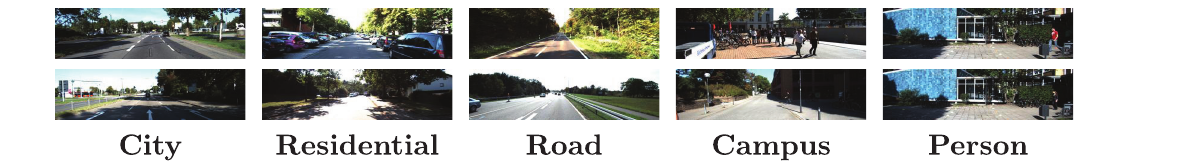
\includegraphics[width=\textwidth, height=0.4\textheight, keepaspectratio]{figs/kitti.png}
			\caption{KITTI}
		\end{figure}
		\begin{figure}
			\centering
			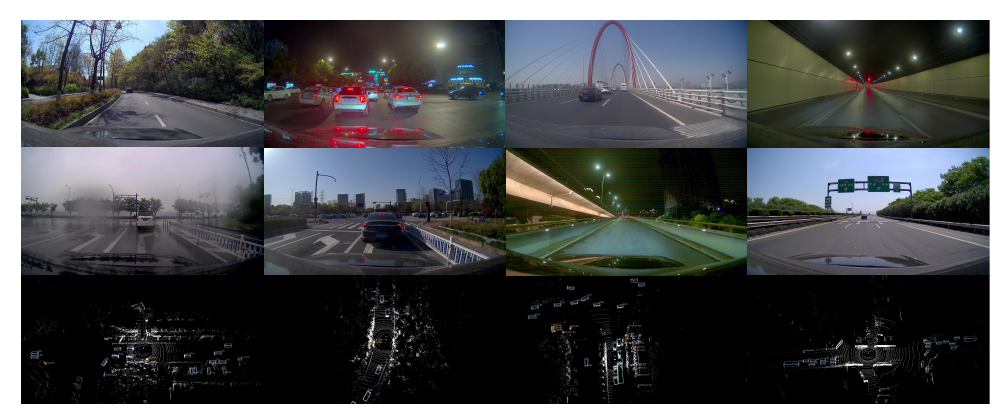
\includegraphics[width=\textwidth, height=0.25\textheight, keepaspectratio]{figs/once.png}
			\caption{ONCE}
		\end{figure}

		\column{0.4\textwidth}
		% \begin{figure}
		% 	\centering
		% 	\includegraphics[width=\textwidth, height=0.25\textheight, keepaspectratio]{figs/argoverse.png}
		% 	\caption{Argoverse 2}
		% \end{figure}
		\begin{figure}
			\centering
			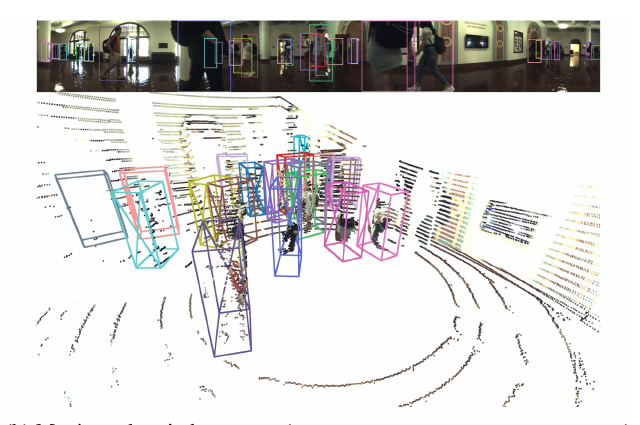
\includegraphics[width=\textwidth, height=0.4\textheight, keepaspectratio]{figs/jrdb.png}
			\caption{JRDB}
		\end{figure}
		\begin{figure}
			\centering
			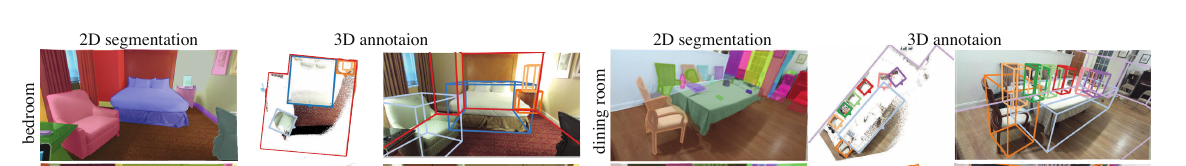
\includegraphics[width=\textwidth, height=0.4\textheight, keepaspectratio]{figs/sunrgbd.png}
			\caption{SUN RGB-D}
		\end{figure}
	\end{columns}
\end{frame}

\section{Work Setting}
\begin{frame}{Work Setting}
	\begin{columns}[T]
		\column{0.5\textwidth}
		\textbf{Camera}
		\begin{itemize}
			\item Intel RealSense model D435I
			\item Indoor office environment
			\item Normal overhead or natural lighting
		\end{itemize}

		\vspace{0.3cm}
		\textbf{Goal}
		\begin{itemize}
			\item Detect faces and people in the point cloud
			\item Apply blurring to protect privacy
		\end{itemize}

		\column{0.5\textwidth}
		\textbf{Camera Specifications}
		\begin{itemize}
			\item Resolution:1280x720
			\item Depth FoV: H:87,V:58
			\item FPS:30
		\end{itemize}
		\vspace{0.3cm}
		\begin{figure}
			\centering
			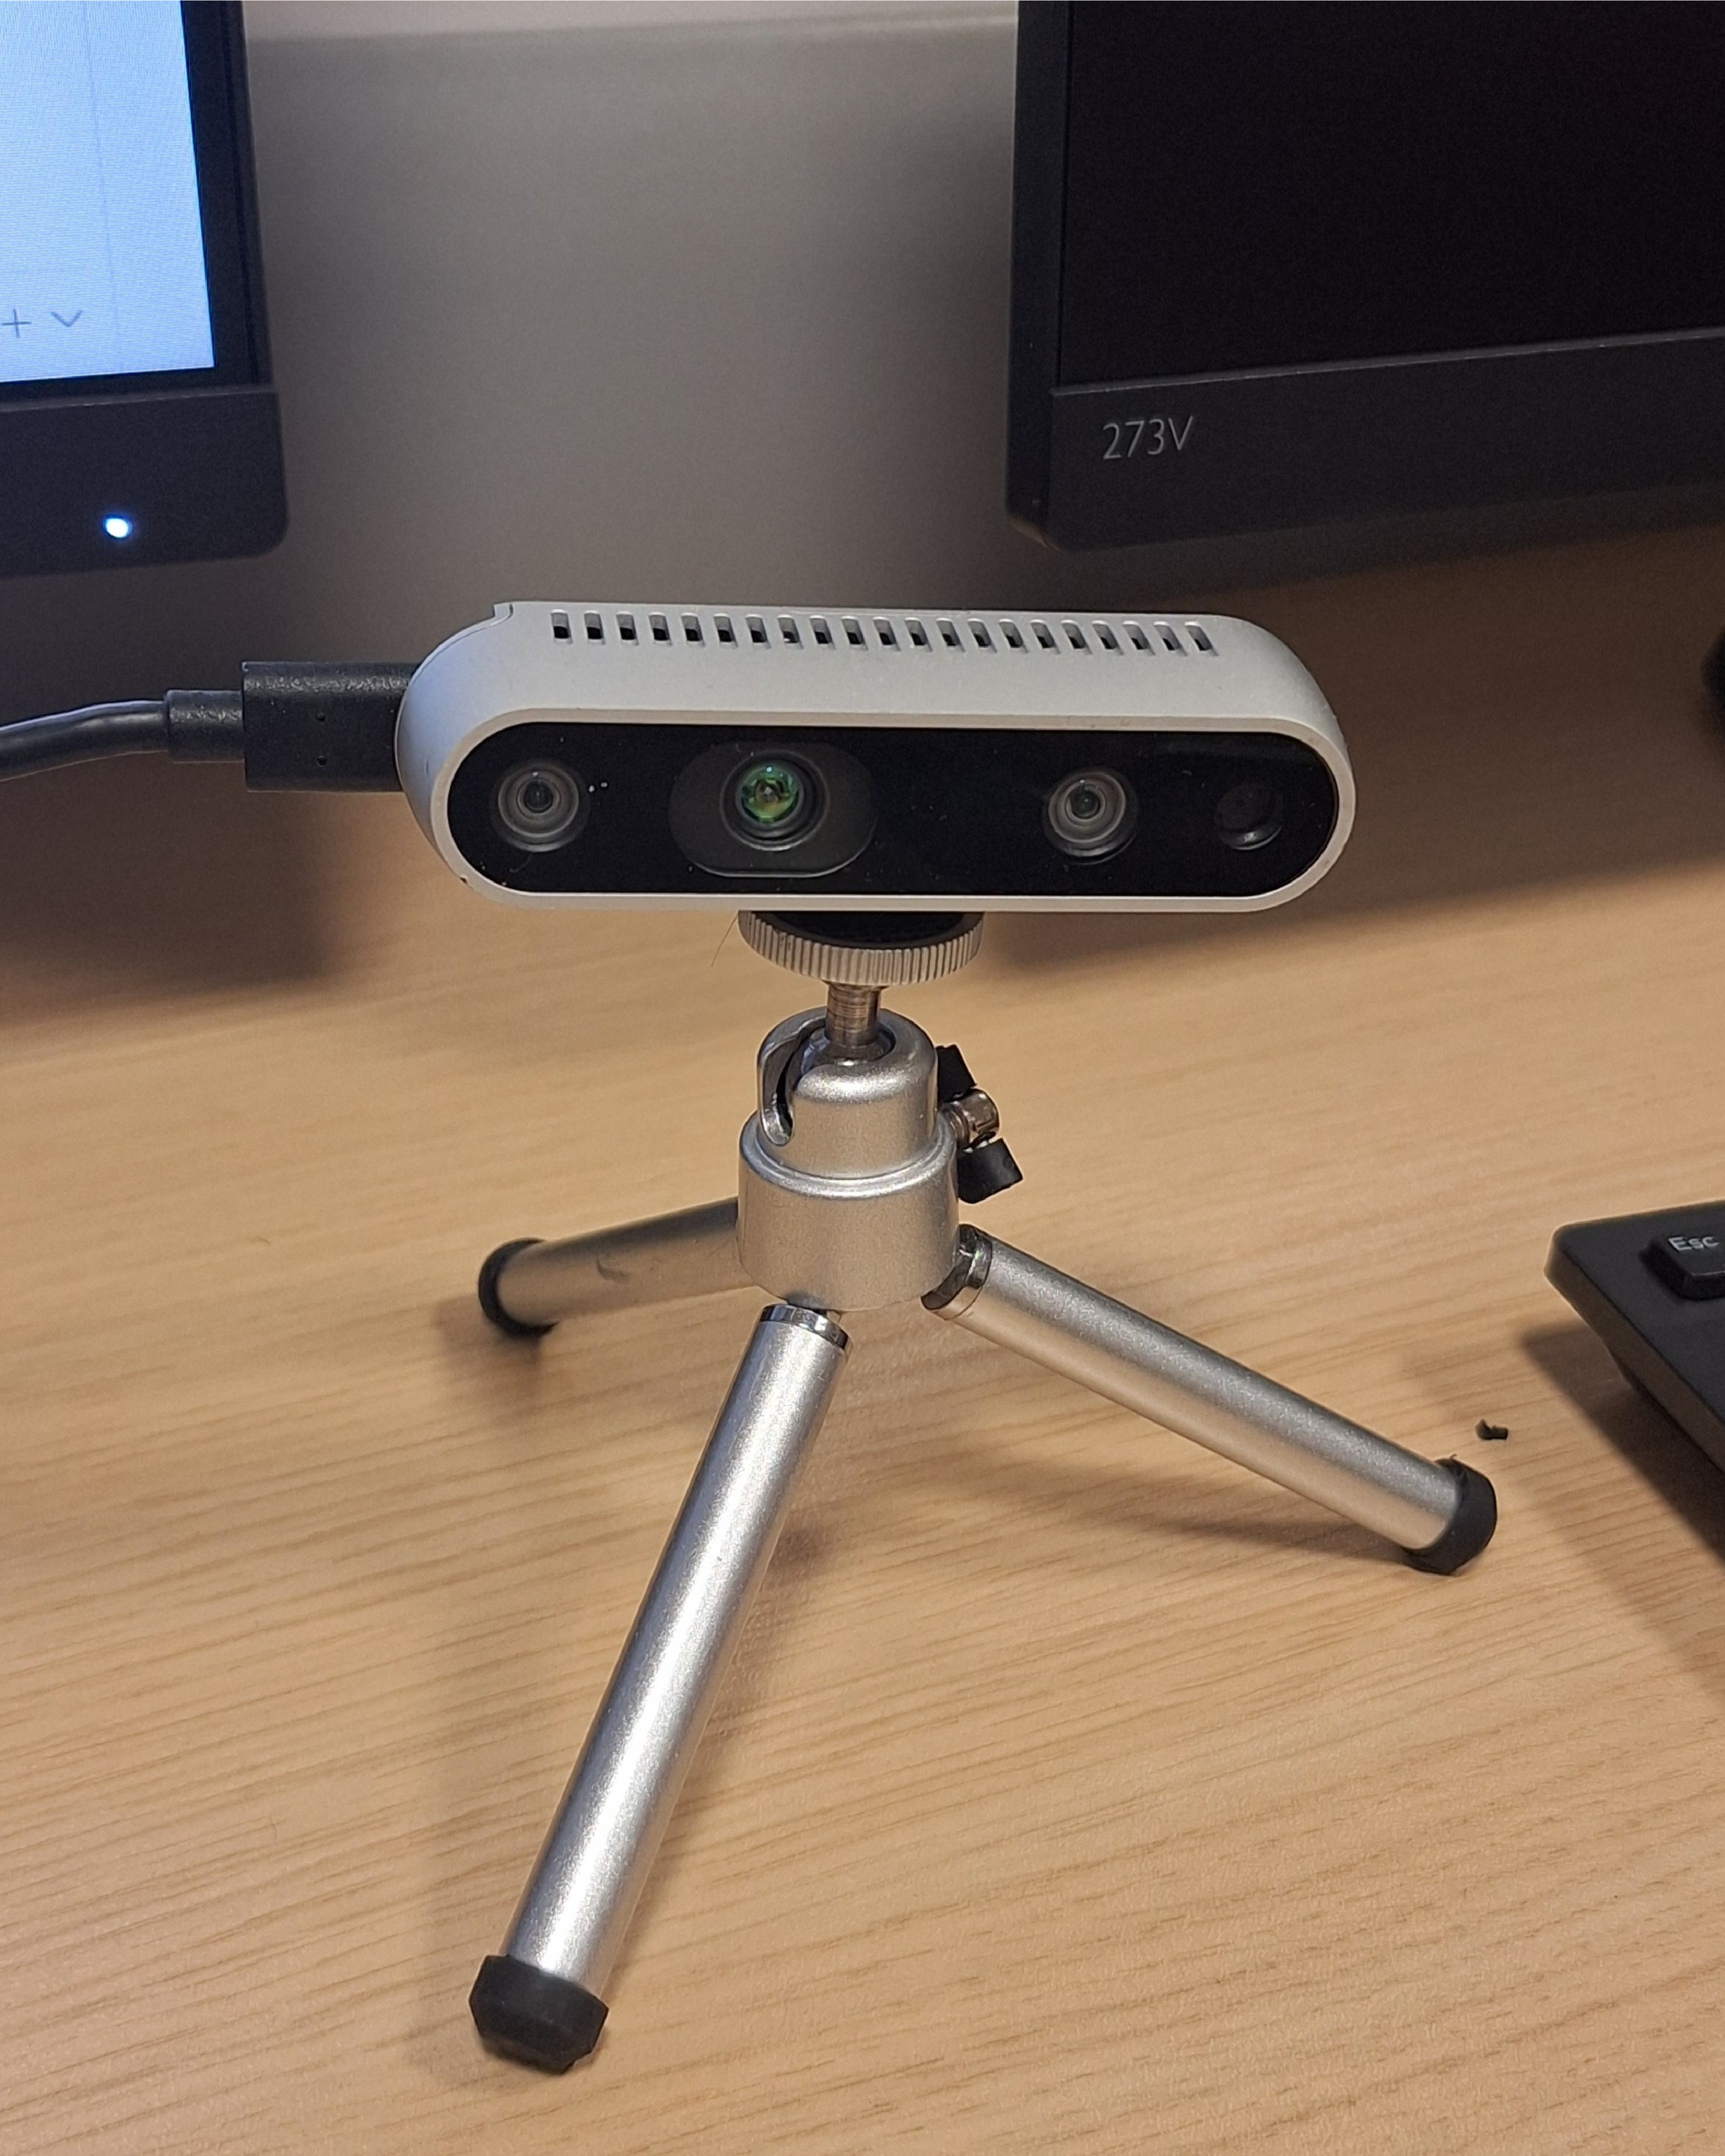
\includegraphics[width=0.7\textwidth]{figs/Realsense-Camera.pdf}
		\end{figure}
	\end{columns}
\end{frame}

\section{Software Demonstration}
\begin{frame}{Demonstration}
	\begin{enumerate}
		\item Reads depth and color frames at each iteration
		\item Face and people detection runs on each frame
		\item Detection results passed to the rendering engine
		\item Blurring effects are applied and the point cloud is rendered
	\end{enumerate}

	\vspace{0.3cm}
	\begin{block}{Experimentally implemented}
		\begin{itemize}
			\item Semantic segmentation using RandLaNet and KPFCNN (unsuccessful)
			\item 3D object detection with PointPillars (unsuccessful)
		\end{itemize}
	\end{block}
\end{frame}
\begin{frame}{Demonstration --- Results}
	\begin{columns}[T]
		\column{0.33\textwidth}
		\begin{figure}
			\centering
			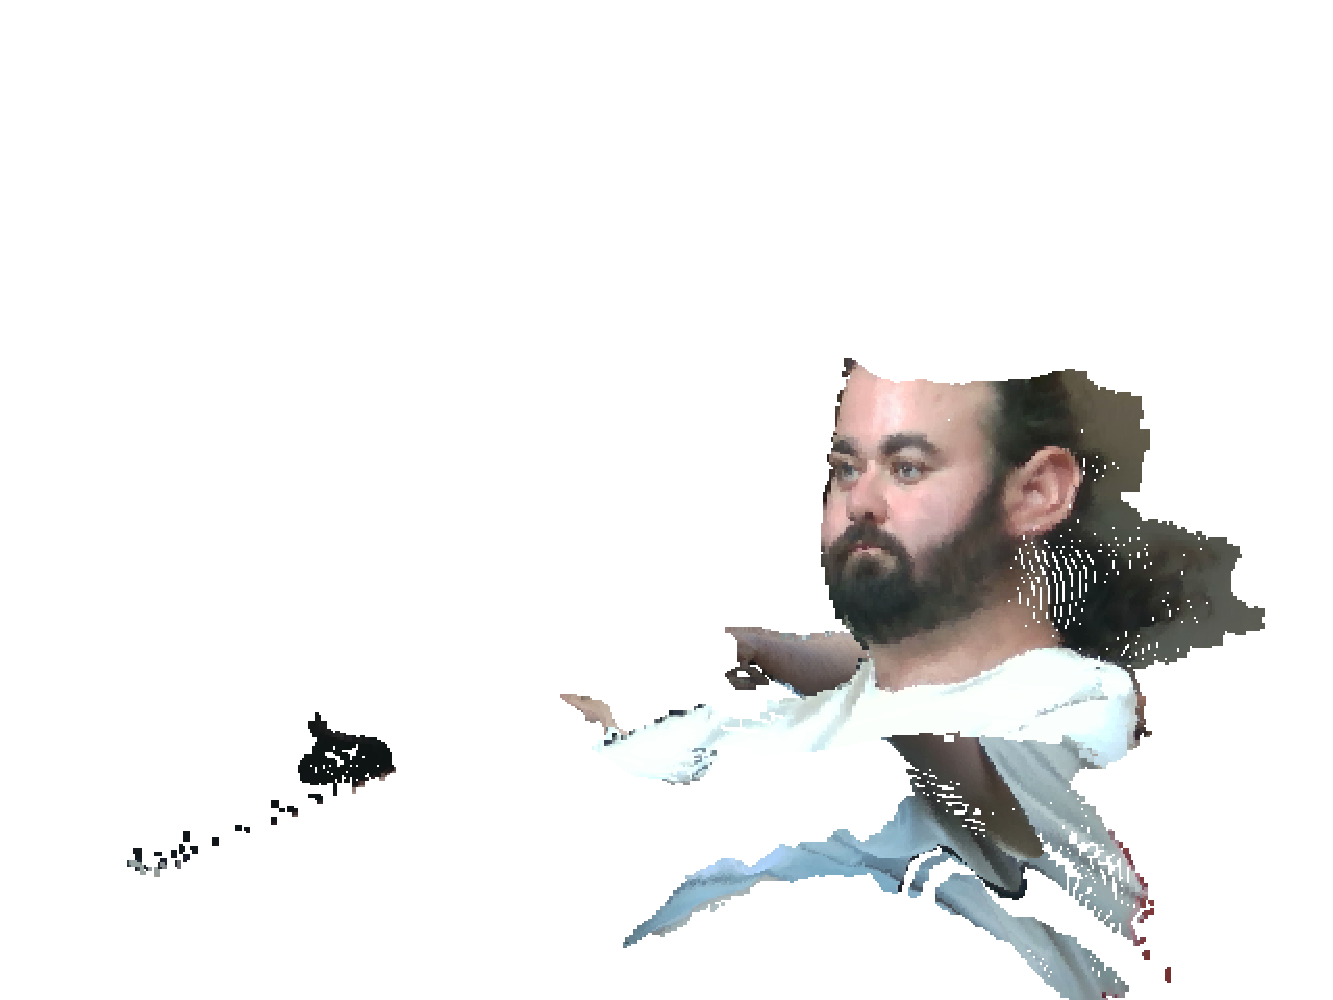
\includegraphics[width=\textwidth]{figs/Pointcloud-Face-Without-Blur.pdf}
			\caption{Without blurring}
		\end{figure}

		\column{0.33\textwidth}
		\begin{figure}
			\centering
			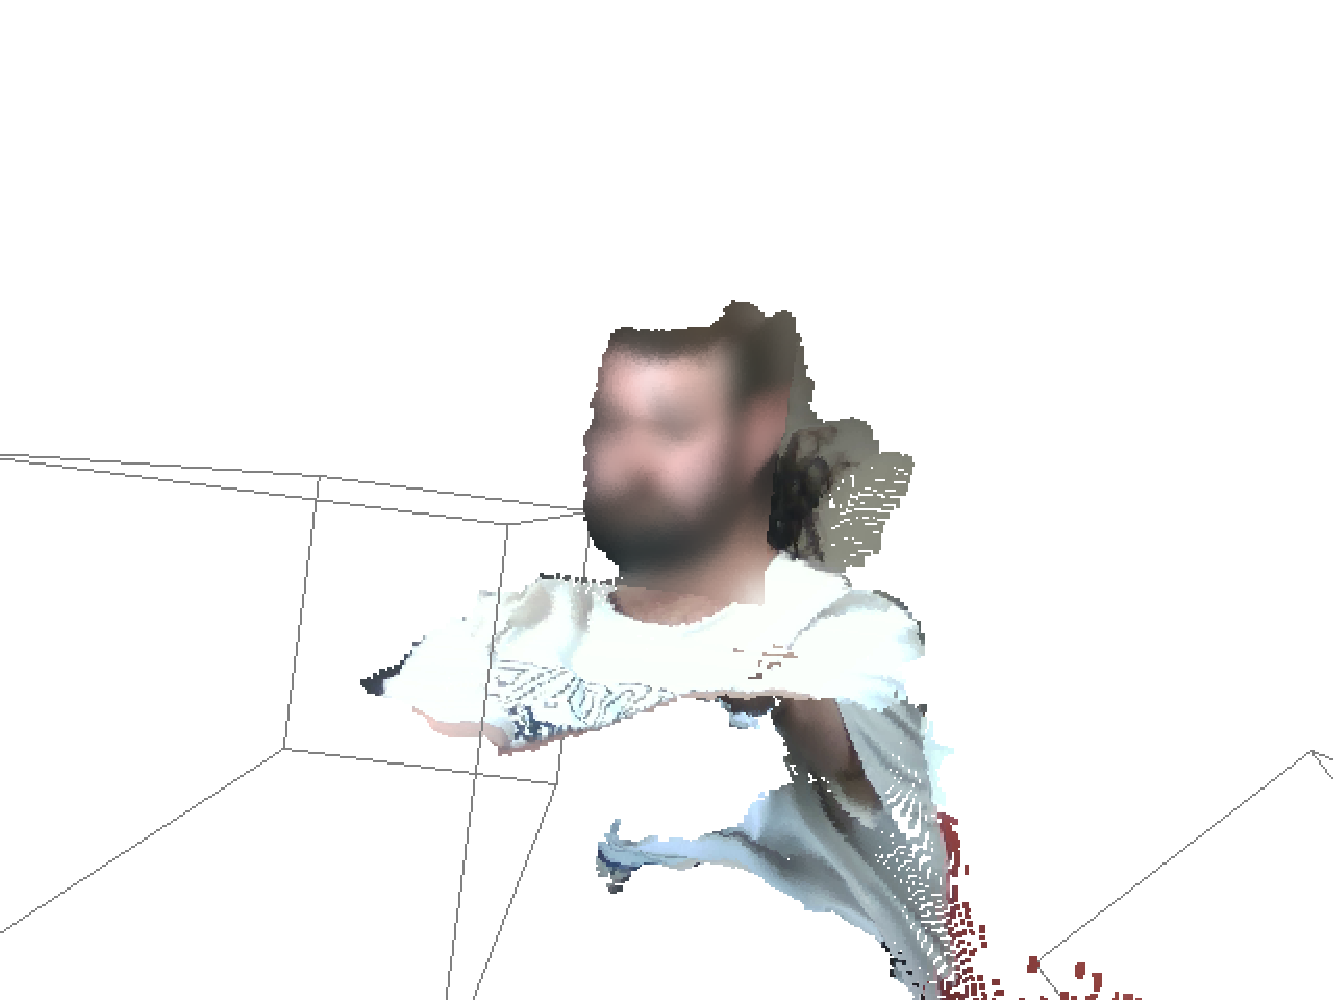
\includegraphics[width=\textwidth]{figs/Face-Blurred-With-2D-Detection-And-Blur.pdf}
			\caption{With blurring}
		\end{figure}

		\column{0.33\textwidth}
		\begin{figure}
			\centering
			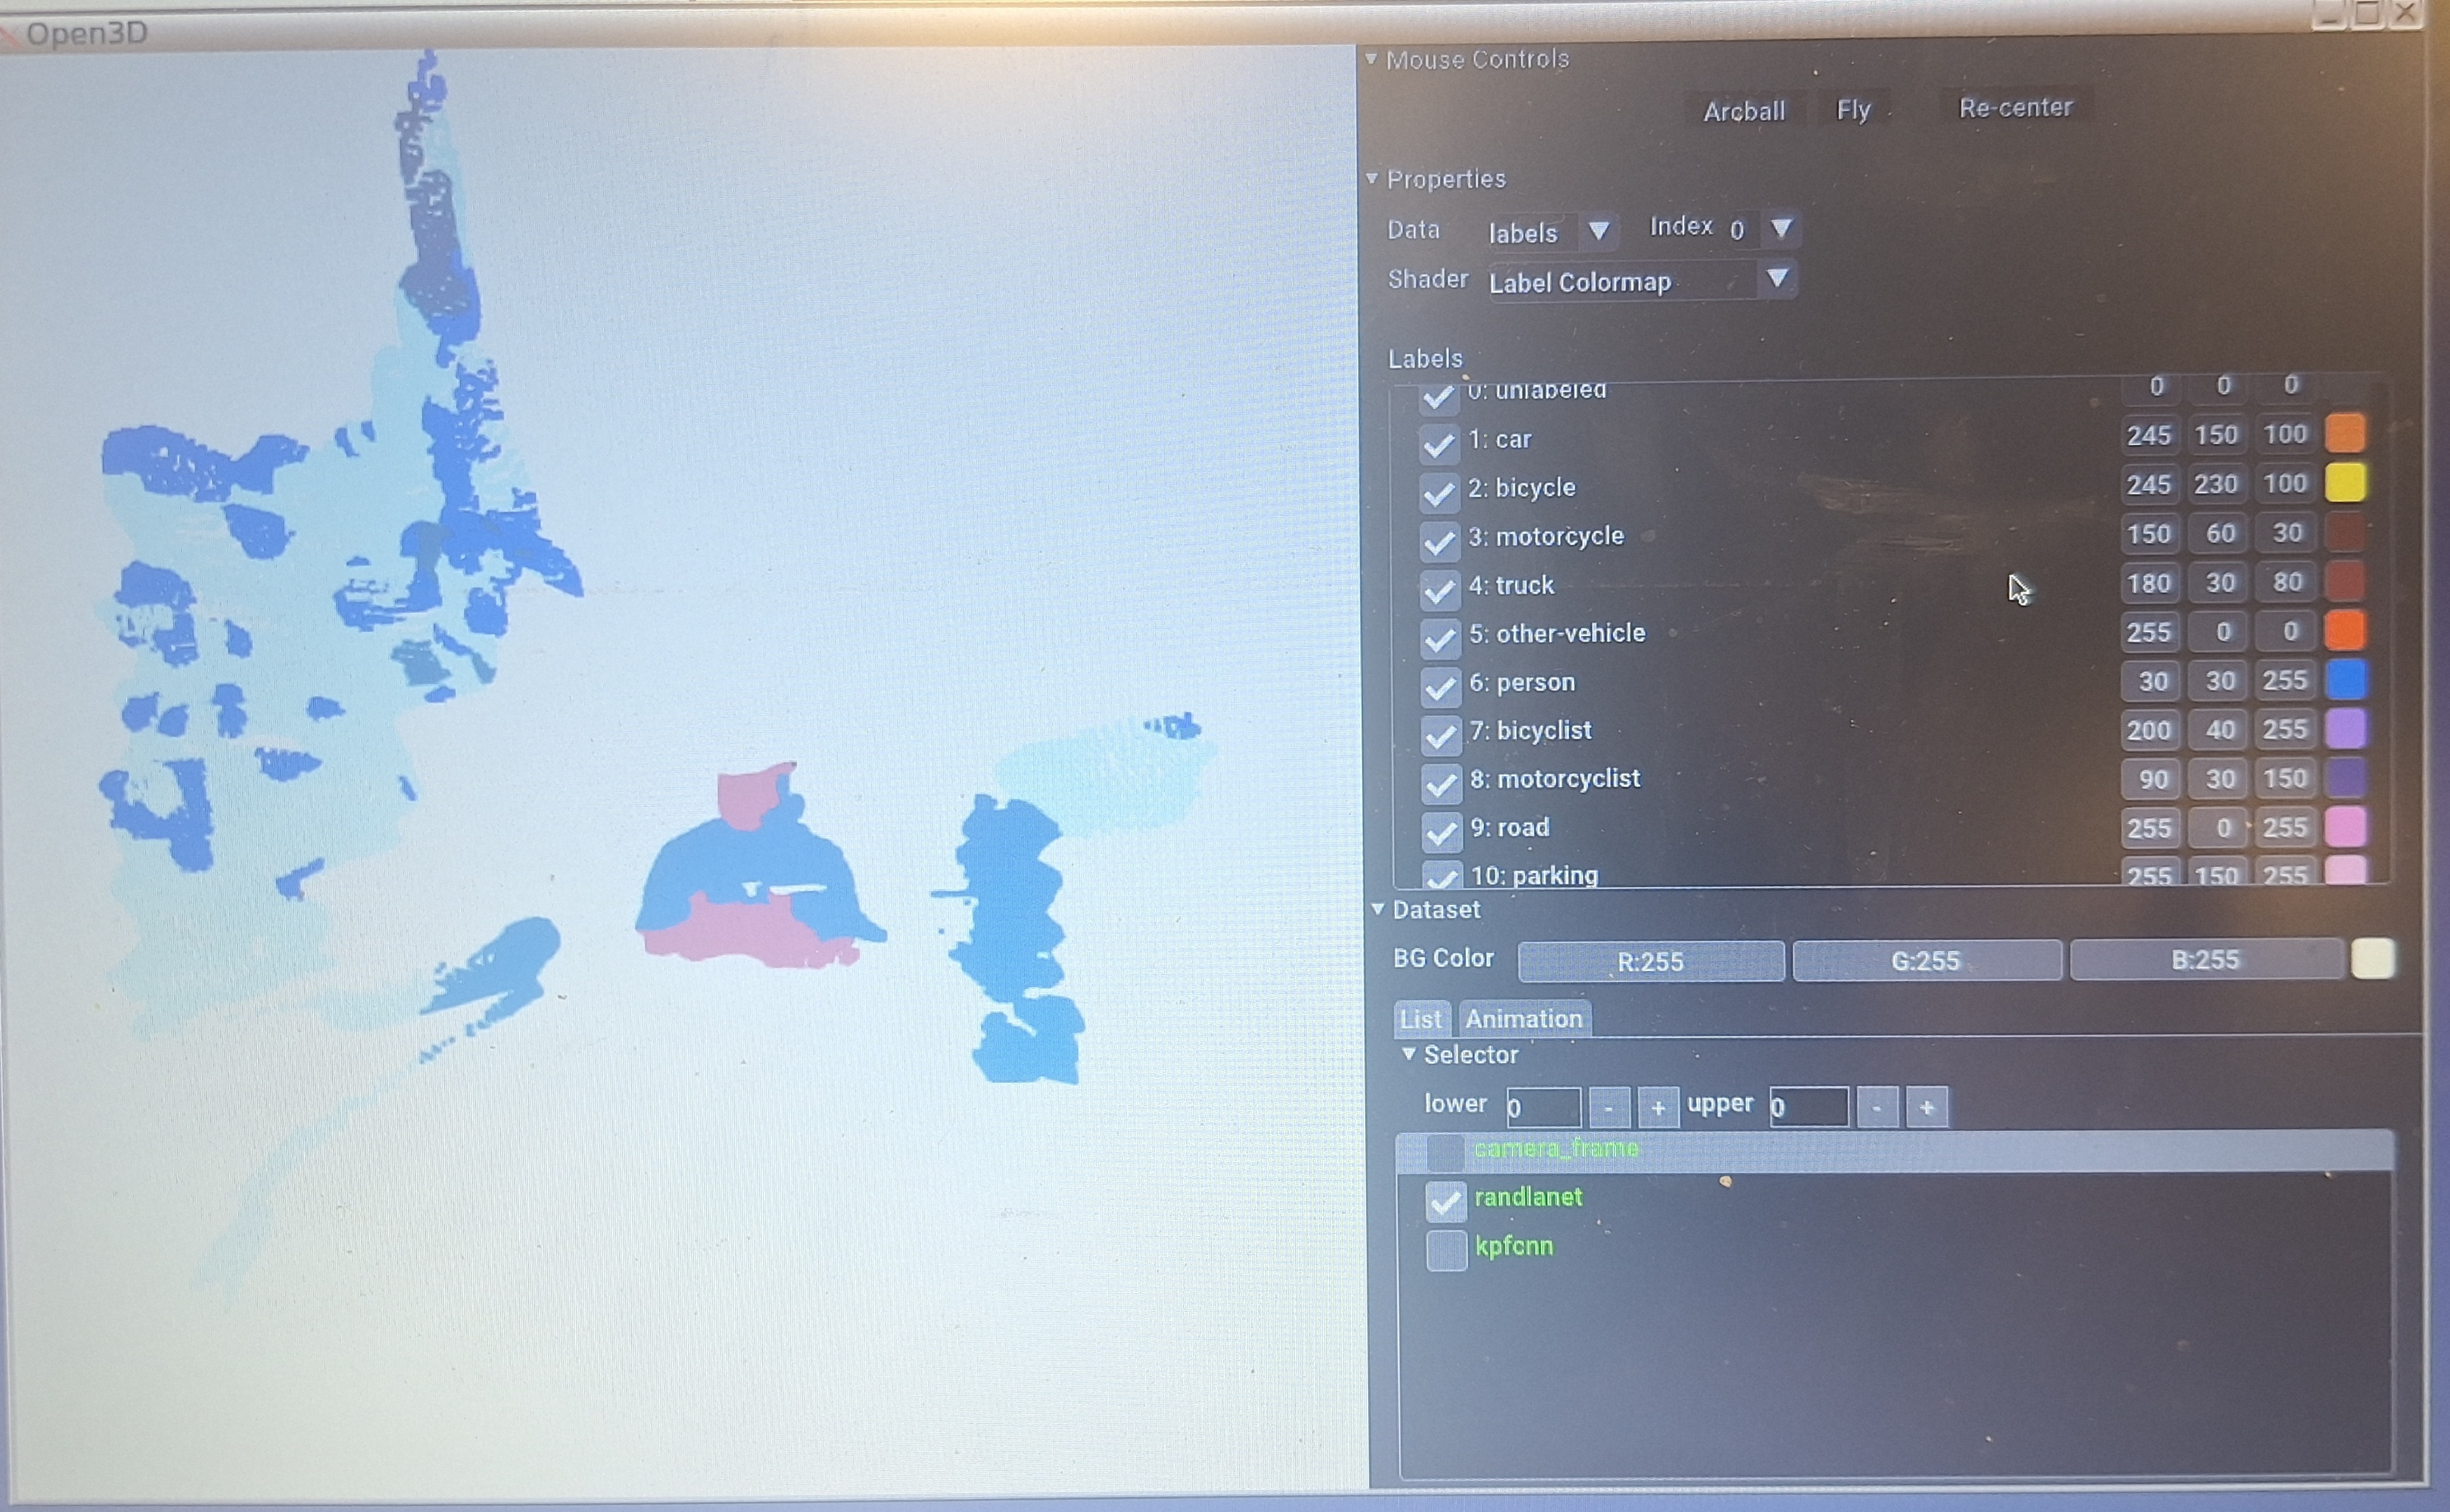
\includegraphics[width=\textwidth]{figs/Semantic-Segmentation-Example.pdf}
			\caption{Semantic segmentation}
		\end{figure}
	\end{columns}
\end{frame}

\section{Implementation}
\begin{frame}{Implementation}
	\begin{columns}[T]
		\column{0.55\textwidth}
		\textbf{Language \& Motivation}
		\begin{itemize}
			\item Python for AI library compatibility
			\item C++ would enable more features and be faster but development time
			      would be significantly more
		\end{itemize}

		\vspace{0.3cm}
		\textbf{Libraries Used}
		\begin{itemize}
			\item \textbf{Open3D}: point cloud processing and visualisation
			\item \textbf{Open3D-ML}: AI tasks (detection, segmentation)
			\item \textbf{OpenCV}: 2D face detection, MobileNet-SSD
			\item \textbf{Pyrealsense2}: RealSense camera interface
		\end{itemize}

		\column{0.5\textwidth}
		\textbf{Tools Considered but Not Used}
		\begin{itemize}
			\item \textbf{OpenPCDet}: required CUDA, unavailable
			\item \textbf{MMDetection3D}: integration issues
			\item \textbf{Learning3D}: limited model support
		\end{itemize}
	\end{columns}
\end{frame}
\begin{frame}{System Architecture}
	\begin{columns}[T]
		\column{0.5\textwidth}
		\textbf{Architecture Overview}
		\begin{itemize}
			\item CameraReader interface(could support streaming and other hardware in the future)
			\item EventBus
			\item EffectsManager (makes it easier to integrate extra features/models for detection)
		\end{itemize}


		\column{0.5\textwidth}
		\begin{figure}
			\centering
			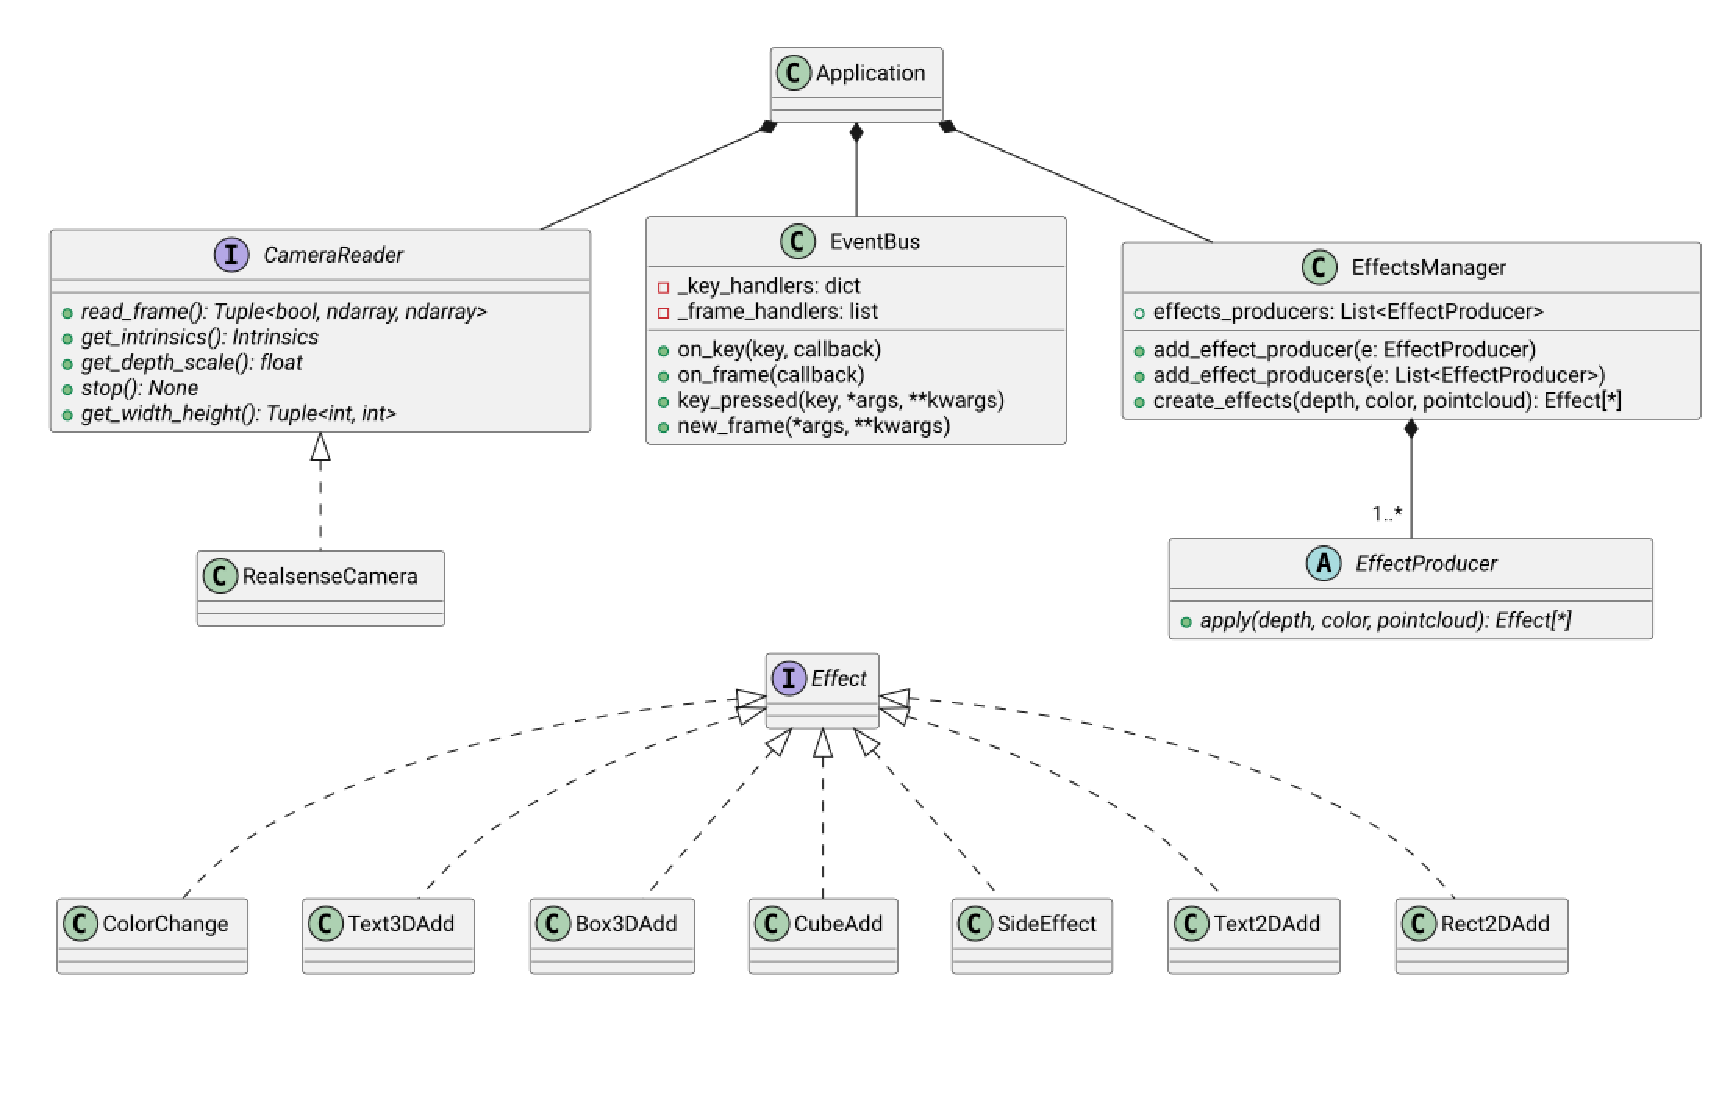
\includegraphics[width=\textwidth]{figs/Uml-Diagram-Thesis-Final.pdf}
			\caption{UML class diagram}
		\end{figure}
	\end{columns}
\end{frame}
\section{Discussion}
\begin{frame}{Discussion}
	\begin{itemize}
		\item Face detection != Face recognition, lots of work in 3D face recognition, less on 3D face detection.
		\item Traffic settings and outdoor scenes receive most of the research attention.
		\item Implementing operations on point clouds is more complex.
		\item Point cloud and 3D object detection ecosystem in python is not production ready.
		\item There is a research/software gap for an end-to-end pipeline that anonymizes of 3D videos.
	\end{itemize}
\end{frame}

\begin{frame}[allowframebreaks]{Bibliography}
	\bibliographystyle{plain}
	\bibliography{MSc-Thesis}
\end{frame}

\begin{frame}[plain]
	\centering
	\vspace{2cm}
	{\Huge\bfseries Thank You}

	\vspace{1cm}
	{\Large Questions?}
\end{frame}


\end{document}
